\chapter{Special-purpose components}
\index{Library!Components!misc}

The chapter deals with components that are not easily included
in any of the other chapters because of their special nature,
but which are still part of the \MCS\ system.

One part of these components deals with splitting simulations
into two (or more) stages. For example, a guide system is often
not changed much, and a long simulation of neutron rays
``surviving'' through the guide system could be reused
for several simulations of the instrument back-end, speeding up
the simulations by (typically) one or two orders of magnitude.
The components for doing this trick is {\bf Virtual\_input} and
{\bf Virtual\_output}, which stores and reads neutron rays, respectively.

Other components perform the simulation of the instrument
resolution functions. These are {\bf Res\_sample} and {\bf TOF\_Res\_sample},
which are to be
placed at the sample position, and {\bf Res\_monitor}, that should
be localized at the position of the instrument detector.

{\bf Progress\_bar} is a simulation utility that displays the simulation
status, but assumes the form of a component.

\newpage
\section{Virtual\_output: Saving the first part of a split simulation}
\label{virtual_output}
\index{Sources!Virtual source, recording neutron events}

\component{Virtual\_output}{System}{filename}{buffer-size, type}{}

The component {\bf Virtual\_output} stores the neutron ray parameters
at the end of the first part of a split simulation. The idea is to let the
next part of the split simulation be performed by another instrument file,
which reads the stored neutron ray
parameters by the component {\bf Virtual\_input}.

All neutron ray parameters are saved to the output file, which is by default
of ``text'' type, but can also assume the binary formats
``float'' or ``double''. The storing of neutron rays continues until the
specified number of simulations have been performed.

\verb+buffer-size+ may be used to limit the size of the output file, but
absolute intentities are then likely to be wrong.
Exept when using MPI, we recommend to use the default value of zero, saving all neutron rays.
The size of the file is then controlled indirectly with the general $ncounts$ parameter.


\section{Virtual\_input: Starting the second part of a split simulation}
\label{virtual_input}
\index{Sources!Virtual source from stored neutron events}

\component{Virtual\_input}{System}{filename}{repeat-count, type}{}

The component {\bf Virtual\_input} resumes a split simulation where the
first part has been performed by another instrument and the neutron ray
parameters have been stored by the component {\bf Virtual\_output}.

All neutron ray parameters are read from the input file, which is by default
of ``text'' type, but can also assume the binary formats
``float'' and ``double''. The reading of neutron rays continues until the
specified number of rays have been simulated or
till the file has been exhausted. If desirable, the input file
can be reused a number of times, determined by the optional parameter
``repeat-count''. This is only useful if the present simulation makes use of
MC choices, otherwise the same outcome will result for each repetition of the
simulation (see Appendix \ref{s:MCtechniques}).

Care should be taken when dealing with
absolute intensities, which will be correct only
when the input file has been exhausted at least once.

The simulation ends with either the end of the repeated file counts,
or with the normal end with $ncount$ \MCS simulation events. We recommend to
control the simulation on \verb+repeat-count+ by using
a very larger ncount value.


\newpage
\section{Res\_sample: A sample-like component for resolution calculation}
\label{s:res_sample}
\index{Samples!Resolution function, sample for}

\component{Res\_sample}{(System); Alan Tennant, HMI}{$r$, $r$, $h$, $r_{\rm focus}$, $x_{\rm target}$, $y_{\rm target}$, $z_{\rm target}$, $E_0$, $\Delta E$ }{$x_w$, $y_h$, $z_d$, $x_{\rm focus}$, $y_{\rm focus}$, $a_{\rm v, focus}$, $a_{\rm h, focus}$, target index}{}

The component \textbf{Res\_sample} scatters neutron rays isotropically
in direction and uniformly in energy.
Regardless of the state of the incoming neutron ray,
all directions and energies for the scattered ray have the same probability,
within specified intervals.

The component is meant
for computation of the resolution function, but may also be used
for test and debugging purposes. For actual calculations of the resolution
function, {\bf Res\_sample} should be used
together with \textbf{Res\_monitor}, described in
section~\ref{s:res_monitor}.

The shape of {\rm Res\_sample} is either a hollow cylinder
or a rectangular box.
The hollow cylinder shape is
specified with the outer radius, $r$ and thickness,
respectively, and the height, $h$.
If these parameters are unspecified,
the shape is instead a box of dimensions $x_w$, $y_h$, and $z_d$.
%
%\begin{figure}[htbp]
%  \begin{center}
%        \psfrag{ri}[c][c]{\textit{radius\_i}}
%        \psfrag{ro}[c][c]{\textit{radius\_o}}
%        \psfrag{h}[c][c]{\textit{h}}
%        \psfrag{bri}[c][c]{\textit{radius\_i}}
%        \psfrag{bro}[c][c]{$-\textit{radius\_o}$}
%        \psfrag{bh}[c][c]{\textit{h}}
%        \psfrag{X}[c][c]{\textit{X}}
%        \psfrag{Y}[c][c]{\textit{Y}}
%        \psfrag{Z}[c][c]{\textit{Z}}
%        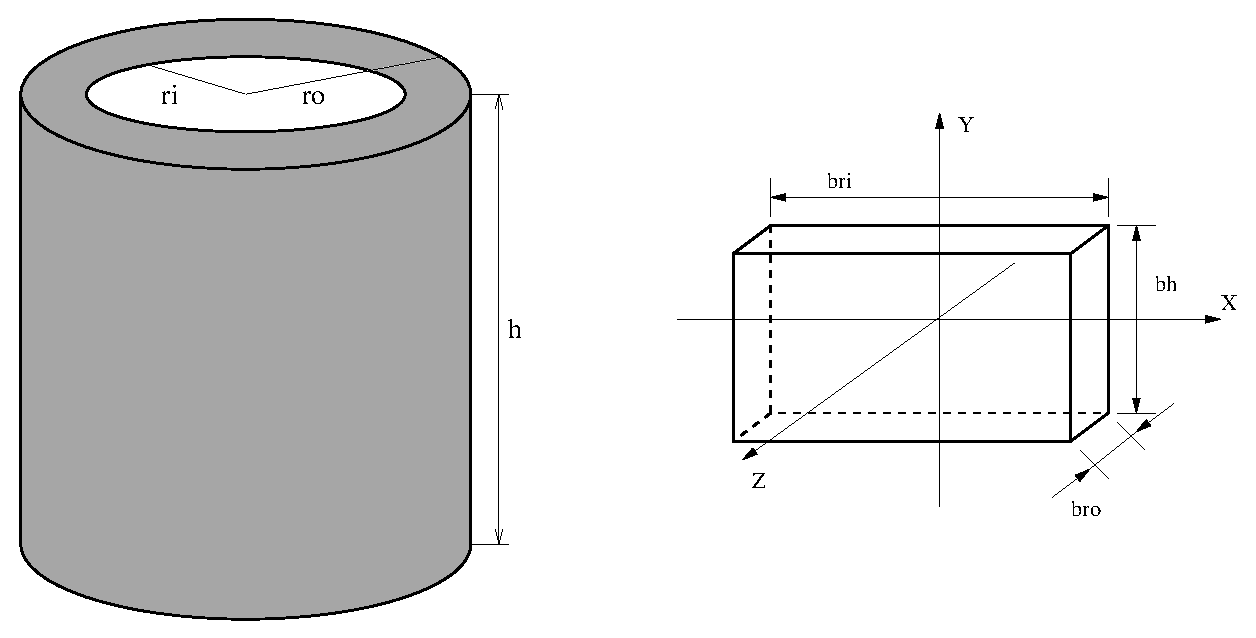
\includegraphics[width=0.9\textwidth]{figures/res_sample}
%    \caption{The two possible shapes of the \textbf{Res\_sample} component.}
%    \label{f:res_sample}
%  \end{center}
%\end{figure}
%
The component only propagates neutron rays that are scattered;
other rays are absorbed. The scattering probability is proportional to the neutron
flight path length inside the sample, to make a true volume weighting
of the sample. The reason for this is that the resolution
function of an instrument is independent of any sample properties
such as scattering and absorbtion cross sections but will in general
depend on sample size and shape.

The point of scattering inside the sample is chosen uniformly
along the neutron flight path inside the sample, and the scattered
neutron ray is given a random energy and direction. This energy is selected in
the interval $[E_0-\Delta E; E_0+\Delta E]$ which hence must be
chosen large enough to cover all interesting neutron energies.
Similarly, the scattered
direction is chosen in a user-specified range,
either within a sphere of radius $r_{\rm focus}$, within a rectangular
target with measures $(x_{\rm focus}, y_{\rm focus})$
or in the specified angular range. This target is positioned at the $x_{target}$, $y_{target}$, $z_{target}$ point in space, or using the target\_index for which e.g. 1 is the further component, -1 is the previous, etc...

A special feature, used when computing resolution functions, is that the
component stores complete information about the scattering event in the
output parameter \textit{res\_struct}. The information includes initial
and final wave vectors, the coordinates of the scattering point, and the
neutron weight after the scattering event. From this information the
scattering parameters $({\bf Q}, \omega)$ can be recorded
for every scattering event and used to compute the resolution function.
For an example of using the
information in the output parameter, see the description of the
\textbf{Res\_monitor} component in section~\ref{s:res_monitor}.



% Emacs settings: -*-mode: latex; TeX-master: "manual.tex"; -*-

\section{TOF\_Res\_sample: A sample-like component for TOF resolution calculation}
\label{s:tof_res_sample}

\component{TOF\_Res\_sample}{System}{$r_{\rm i}$, $r_{\rm o}$, $h$, $r_{\rm focus}$, $x_{\rm target}$, $y_{\rm target}$, $z_{\rm target}$, $t_0$, $\Delta t$ }{$x_w$, $y_h$, $z_t$, $x_{\rm focus}$, $y_{\rm focus}$, $a_{\rm v, focus}$, $a_{\rm h, focus}$, target index}{}

The component \textbf{TOF\_Res\_sample} scatters neutron rays isotropically
in position within a specified angular range. 
As for {\bf Res\_sample}, this component is meant
for computation of the resolution function, but in this case for one time bin in a
time-of-flight (TOF) instrument. The component selects uniformly the neutron 
energy so that neutron arrival time at the TOF detector lies within one time bin,
specified by $t_0$ and $\Delta t$.
For actual calculations of the resolution
function, {\bf TOF\_Res\_sample} should be used
together with \textbf{Res\_monitor}, described in
section~\ref{s:res_monitor}.

The shape of {\bf TOF\_Res\_sample} is either a hollow cylinder
or a rectangular box. 
The hollow cylinder shape is
specified with the inner and outer radius, $r_{\rm i}$ and $r_{\rm o}$,
respectively, and the height, $h$.
If these parameters are unspecified,
the shape is instead a box of dimensions $x_w$, $y_h$, and $z_t$.
%See figure~\ref{f:res_sample}.\par

The component only propagates neutron rays that are scattered; 
other rays are absorbed. 
As for {\bf Res\_sample}, the scattering probability is proportional to the neutron
flight path length inside the sample.
The point of scattering in the sample is chosen uniformly
along the neutron flight path inside the sample, and the scattered
direction is chosen in a user-specified range,
either within a sphere of radius $r_{\rm foc}$, within a rectangular
target with measures $(x_{\rm focus}, y_{\rm focus})$
or in the specified angular range. 
This target is positioned at the $x_{target}$, $y_{target}$, $z_{target}$ 
point in space, or using target\_index.

This component stores complete information about the scattering event in the
output parameter \textit{res\_struct}, see {\bf Res\_Sample}. 


\section{Res\_monitor: The monitor for resolution calculation}
\label{s:res_monitor}
\index{Monitors!Resolution monitor|see{Samples/Resolution function}}

\component{Res\_monitor}{(System); Alan Tennant, HMI}{$x_{\rm min}$, $x_{\rm max}$, $y_{\rm min}$, $y_{\rm max}$, filename, res\_sample, buffer size}{$x_w$, $y_h$, $z_t$, options}{}

The component {\bf Res\_monitor} is used for calculating the
resolution function of a particular instrument with detector of the
given shape, size, and position.
The shape of {\bf Res\_monitor} is by default rectangular,
but can be a box, a sphere, a disk, or a cylinder,
depending on the parameter ``options''.
The component works like a normal monitor, but
also records all scattering events and stores
them to a file that can later be read by 
the \MCS\ frontend tool \verb+mcresplot+.

For time-of-flight (TOF) instruments, {Res\_monitor} should be understood 
as giving the resolution of one time bin of the TOF-detector only; 
the bin properties being specified in the preceding {\bf TOF\_Res\_sample}.

As described in section~\ref{s:res_sample},
the {\bf Res\_monitor} should be used in connection with one of the
components {\bf Res\_sample} or {\bf TOF\_Res\_sample}, 
the name of which should be passed as an
input parameter to \textbf{Res\_monitor}. For example
\begin{verbatim}
    COMPONENT mysample = Res_sample( ... )
    ...
    COMPONENT det = Res_monitor(res_sample_comp = mysample, ...)
    ...
\end{verbatim}

The output file is in ASCII format, one line per scattering event, with
the following columns:
\begin{itemize}
\item ${\bf k}_{\rm i}$, the three components of the initial wave vector.
\item ${\bf k}_{\rm f}$, the three components of the final wave vector.
\item ${\bf r}$, the three components of the position of the scattering
  event in the sample.
\item $p_{\rm i}$, the neutron weight just after the scattering event.
\item $p_{\rm f}$, the relative neutron weight adjustment from sample to
  detector (so the total weight in the detector is $p_{\rm i}p_{\rm f}$).
\end{itemize}
From ${\bf k}_{\rm i}$ and ${\bf k}_{\rm f}$, we may compute 
the scattering parameters 
$\kappa = {\bf k}_{\rm i} - {\bf k}_{\rm f}$ and 
$\hbar \omega = \hbar^2/(2 m_{\rm n})({\bf k}_{\rm i}^2 - {\bf k}_{\rm f}^2)$.
The vectors are given in the local coordinate system of the resolution
sample component. The wave vectors are in units of $\mbox{\AA}^{-1}$, the
energy transfer in meV.

The output parameters from {\bf Res\_monitor}
are the three count numbers, \textit{Nsum}, \textit{psum},
and \textit{p2sum}, and the handle \textit{file} of the output file.


\newpage
\section{Progress\_bar: Simulation progress and automatic saving}
\component{Progress\_bar}{System}{percent, flag\_save, profile}{}{}
\label{s:progress-bar}
\index{Simulation progress bar}

This component displays the simulation progress and status
but does not affect the neutron parameters.
The display is updated in regular intervals of the full simulation;
the default step size is 10 \%, but it may be changed using
the \verb+percent+ parameter (from 0 to 100).
The estimated computation time is displayed at the begining
and actual simulation time is shown at the end.

Additionally, setting the \verb+flag_save+ to 1 results in
a regular save of the data files during the simulation.
This means that is is possible to view the data before the end
of the computation, and have also a trace of it in case of
computer crash. The achieved percentage of the simulation is stored in these temporary
data files. Technically, this save is equivalent to sending regularly
a USR2 signal to the running simulation.

The optional 'profile' parameter, when set to a file name, will produce the number of statistical events reaching each component in the simulation. This may be used to identify positions where events are lost.

\section{Beam\_spy: A beam analyzer}
\component{Beam\_spy}{System}{}{}{should overlap previous component}
\index{Monitors!Beam analyzer}

This component is at the same time an Arm and a simple Monitor. It analyzes all neutrons reaching it, and computes statistics for the beam, as well as the intensity.

This component does not affect the neutron beam, and does not contain any propagation call. Thus it gets neutrons from the previous component in the instrument description, and should better be placed at the same position, with \verb+AT (0,0,0) RELATIVE PREVIOUS+.